\chapter{CSO迁移：学习的新定义}
\label{chap:cso-migration}

\begin{chapteroverviewbox}
在上一章中，我们完成了一次重要的本体论修正：不再把“复杂度”理解成一种能够像能量一样在系统内部流动的实体，而是把复杂度重新放回描述层，把真正发生变化的对象确定为认知结构对象及其具体承载，即 CSO 与 Agent-CSO。本章将在这一修正之上重新定义“学习”。

本章的基本命题是：\textbf{学习并不首先意味着知识数量增加，也不首先意味着模型参数发生更新；从更一般的智能动力学角度看，学习是同一个或相互关联的 CSO 在智能体内部改变其表示方式、功能位置、运行时间尺度和承载边界的过程。}因此，参数训练、情景记忆写入、知识抽象、技能自动化、程序编译、工具外化、环境改造乃至异常条件下技能重新进入显式认知，都可以被视为 CSO 迁移的不同特殊形式。

我们将把一个具体 Agent 对某一 CSO 的承载状态写成
\[
AgentCSO_A(C,t)
=
\bigl(
C,\,
R_A,\,
F_A,\,
\tau_A,\,
B_A,\,
S_A
\bigr),
\]
其中 $C$ 表示其所对应的认知结构本体，$R_A$ 表示该 Agent 的具体表示，$F_A$ 表示当前功能承载位置，$\tau_A$ 表示该结构发生有效作用的时间尺度，$B_A$ 表示承载边界或载体，$S_A$ 表示激活、潜伏、预测、回忆、程序化等运行状态。本章所谓“迁移”，正是这些坐标在生命周期中的有组织变化。

因此，本章的研究对象不是单一模型的梯度下降，而是一个更广义的问题：

\begin{statementbox}
一个认知结构在一个智能体的一生中，究竟以什么形式、由什么功能、在什么时间尺度、通过什么载体继续存在？
\end{statementbox}

后续关于三相记忆、工作记忆、认知卸载、技能编译、Body Runtime 和功能拓扑学习的讨论，都将在这一迁移理论之上获得统一解释。
\end{chapteroverviewbox}

\begin{figure}[htbp]
\centering
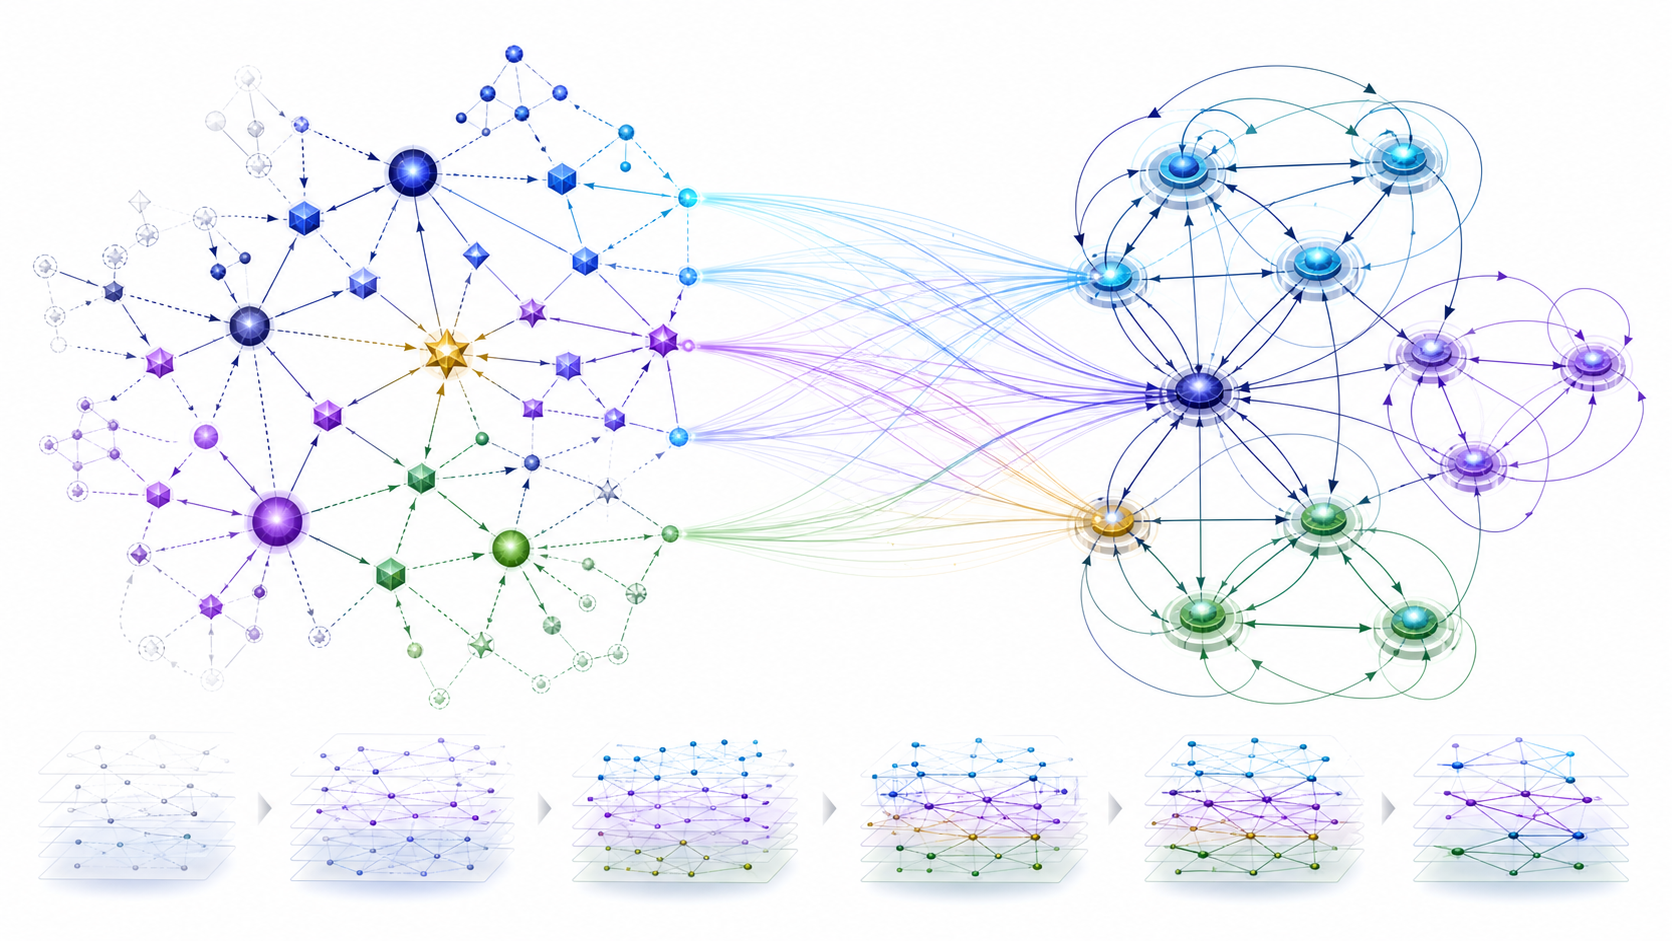
\includegraphics[width=.9\textwidth,height=.38\textheight,keepaspectratio]{images/cognitive-structure-functional-topology.png}
\caption{CSO 在表示、功能、尺度和载体间迁移}
\end{figure}
\section{表示迁移：同一认知结构可以改变其内部编码}

我们首先从最容易被传统机器学习理解的一类变化开始，即表示迁移（representation migration）。当我们说一个 Agent “学会”了某个对象、关系、规则或任务时，最直观的理解往往是其内部表示发生了变化。然而，在本书所采用的 CSO 本体论中，我们必须严格区分“结构本身”与“结构在某个 Agent 内部的表示”。如果 $C$ 表示一个认知结构对象，那么智能体 $A$ 对它的具体实现是
\[
R_A(C,t).
\]
随着经验积累，$C$ 所对应的本体关系可以保持相对稳定，但 $R_A$ 可以经历显著变化。因此，表示迁移首先可以写成
\[
M_R:
R_A(C,t_1)
\longrightarrow
R_A(C,t_2).
\]

这种变化远比“embedding 更新”更加一般。一个幼稚的 Agent 最初可能把“杯子”表示为一组局部视觉特征；进一步学习以后，它可能把杯子表示成具有容器属性、可抓取属性、盛水功能、易碎性和社会用途的关系结构；继续形成经验以后，“杯子”又可能与特定位置、特定人的所有权、特定任务以及操作技能结合。这里并不是外部 CSO 发生了同样程度的变化，而是 Agent 内部对这一 CSO 的表示由低关系密度结构逐渐演化为更加稳定、压缩且可复用的结构。

因此，表示学习可以在 CSO 理论中被理解为
\[
C
\xrightarrow{\pi_A(t_1)}
R_A^{(1)}
\xrightarrow{M_R}
R_A^{(2)}
\xrightarrow{M_R}
\cdots
\xrightarrow{M_R}
R_A^{(n)}.
\]
其中 $\pi_A$ 是 Agent 对 CSO 的具体实现映射。传统表示学习、概念形成、特征抽象、schema formation 等，都可以视为这一过程的不同局部机制。

这里必须注意一个容易产生误解的问题：表示迁移并不意味着后一个表示一定比前一个表示“包含更多信息”。成熟表示往往恰恰具有更高的压缩率。一个初学者为了完成任务可能必须显式保存大量局部步骤，而专家只需要激活少量高阶结构即可重建整个任务空间。因此，表示成熟可能表现为
\[
Dim(R)\downarrow,
\qquad
PredictiveUtility(R)\uparrow,
\]
即显式表示维度下降，但结构解释力和生成能力上升。从信息论角度看，它更接近寻找任务相关的充分统计量，而不是无条件地扩大信息存储量。

我们可以引入一个表示质量泛函
\[
\mathcal Q_R
=
\alpha I(R;Y)
-
\beta I(R;X_{\mathrm{irrelevant}})
-
\gamma Cost(R),
\]
其中 $X$ 表示输入世界状态，$Y$ 表示与当前目标有关的未来状态、动作结果或结构关系，$I(\cdot;\cdot)$ 是互信息，$Cost(R)$ 表示维护该表示所需的认知与计算代价。成熟表示的目标不是简单最大化 $I(R;X)$，因为完整复制世界既不可能也没有必要，而是使 Agent 在有限承载条件下保留对预测和行动真正有价值的结构。

这一点与传统 representation learning、information bottleneck、schema theory 和 predictive representation 有明显的理论关联，但 CSO 迁移的视角比这些理论更广。它关心的不只是“什么表示最好”，还关心：一个表示完成学习以后是否仍然应该停留在原来的功能位置？是否需要进入更慢的结构记忆？是否应当被编译成技能？是否应外化为程序或工具？因此，表示迁移只是整个 CSO 迁移向量中的第一个分量。

我们可以把它形式化为
\[
\mathcal M_{CSO}
=
\left(
M_R,
M_F,
M_\tau,
M_B
\right),
\]
其中 $M_R$ 只描述表示坐标的变化。一个系统即使具有非常强的表示学习能力，如果所有结构始终停留在同一个功能中心、同一个推理速度和同一个内部载体上，它仍然只是一个“表示可塑但组织方式固定”的智能系统。后面的几节将说明，长期智能真正重要的地方恰恰在于表示迁移会逐渐触发更深层的功能、时间尺度和边界迁移。


\section{功能位置迁移：认知结构可以由不同功能承担}

如果表示迁移回答“同一个 CSO 被怎样表示”，那么功能迁移回答的是一个更加关键的问题：\textbf{这个结构现在由系统中的哪一种功能承担？}这一步使学习从传统的参数变化问题进入智能结构动力学问题。

设智能体具有一个功能图
\[
\mathcal G_F
=
(V_F,E_F),
\]
其中
\[
V_F
=
\{F_1,F_2,\ldots,F_n\}
\]
表示不同认知或行动功能，例如显式推理、情景记忆、结构生成、身体控制、工具调用、程序执行和外部查询。对于某一 CSO $C$，在时刻 $t$，其主要承载位置可以表示为
\[
F_A(C,t).
\]
那么功能迁移定义为
\[
M_F:
F_A(C,t_1)
\longrightarrow
F_A(C,t_2).
\]

这一形式能够统一解释大量传统上互相分离的学习现象。一个复杂算术过程在学习早期可能主要由显式工作记忆和推理功能承担：
\[
C_{\mathrm{arith}}
@F_{\mathrm{reasoning}}.
\]
随着重复练习，其部分结构可以被结构记忆和技能系统承担：
\[
C_{\mathrm{arith}}
@F_{\Theta},
\]
进一步可能形成可直接调用的程序：
\[
C_{\mathrm{arith}}
@F_{\mathrm{program}}.
\]
于是，对于同一类任务，我们观察到的主观现象是“想得越来越少”，但这并不意味着能力消失。更准确地说，是
\[
\boxed{
ThinkingLess
\neq
KnowingLess
}
\]
而是
\begin{statementbox}
StructureChangedFunctionalCarrier.
\end{statementbox}

从这个角度看，熟练化（automatization）本质上是一种功能位置下降过程。一个原先需要高层全局闭环处理的 CSO，逐渐迁向更加局部、更快速、更确定的功能闭环：
\[
ExplicitReasoning
\rightarrow
StructuralMemory
\rightarrow
SkillController.
\]
我们可以把这一过程称为功能下迁（functional down-migration）。与之相反，当一个已经熟练的技能遭遇异常情境时，原本由局部系统处理的结构可能重新进入高层显式认知：
\[
SkillController
\rightarrow
h(t)
\rightarrow
ExplicitReasoning.
\]
这就是功能上迁（functional up-migration）。

因此，智能体内部真正存在的不是固定意义上的“高级功能”和“低级功能”，而是具有不同作用范围、自由度和闭环速度的功能区域。高层功能适合处理高不确定性、高新颖性、跨域耦合和结构重构；低层功能适合处理已经稳定、可以局部闭合的重复结构。一个成熟系统应尽量使
\[
\text{GlobalExplicitLoad}
\]
保持稀疏，而让大量稳定结构沉降到局部功能中。

我们可以定义某个 CSO 在功能图上的承载分布
\[
p_C(F_i,t),
\qquad
\sum_i p_C(F_i,t)=1,
\]
而不是假设每个 CSO 永远只有一个唯一承载节点。功能迁移可以表现为该分布中心发生移动：
\[
\bar F_C(t)
=
\sum_i p_C(F_i,t)F_i.
\]
更一般地，如果功能节点不是线性有序的，那么我们应使用图上的概率流
\[
J^{C}_{ij}(t)
\]
表示 CSO $C$ 从功能 $F_i$ 向 $F_j$ 的迁移强度。于是
\[
\dot p_C(F_i,t)
=
\sum_j J^C_{ji}
-
\sum_j J^C_{ij}
+
S_i^C
-
D_i^C.
\]

这一形式与 later chapters 中的功能拓扑学习直接相连：如果某种
\[
F_i\rightarrow F_j
\]
迁移长期、稳定、高价值地重复，那么系统可能逐渐强化相应功能连接，最终产生新的稳定闭环。因此，功能迁移首先是 topology 上的 dynamics，而长期功能迁移的历史沉积又可能变成 dynamics of topology。这也是为什么我们在理论上必须先研究 CSO 在固定拓扑上的迁移，之后才能研究功能拓扑本身怎样学习。


\section{时间尺度迁移：认知结构可以在快变量与慢变量之间移动}

功能位置并不是 CSO 的唯一坐标。即使两个结构由同一种功能承担，它们的有效作用时间尺度也可能完全不同。一个刚刚出现的感觉信号可能只在几十毫秒到几秒范围内具有作用，而一个形成数年的身份结构则可能在极慢尺度上持续约束无数次局部决策。因此，CSO 迁移必须加入时间尺度坐标
\[
\tau_C(t),
\]
并定义
\[
M_\tau:
\tau_C(t_1)
\longrightarrow
\tau_C(t_2).
\]

在我们此前建立的三相记忆体系中，这一过程已经隐含存在：
\[
h
\rightarrow
E
\rightarrow
\Theta.
\]
其中，工作记忆 $h$ 承载的是高速活动结构，情景记忆 $E$ 承载经历轨迹，结构记忆 $\Theta$ 则承载更加缓慢、稳定和具有生成能力的结构。因此，
\[
\tau_h
\ll
\tau_E
\ll
\tau_\Theta.
\]
当一个反复出现的 Agent-CSO 从 $h$ 逐渐进入 $E$，再由 $E$ 被抽象进入 $\Theta$ 时，我们不只是把它“存得更久”，而是在改变它参与未来认知的时间尺度。

这个差异非常重要。高速结构的特点是对当前状态敏感、变化快、能够迅速响应环境；慢速结构的特点是相对稳定、抗噪声、能够作为多个快速过程共同的约束。于是，时间尺度迁移实质上是在改变 CSO 的动力学角色。可以写成
\[
CSO_{\mathrm{fast}}
\rightarrow
CSO_{\mathrm{slow}}
\]
表示稳定化、凝固和长期结构形成；而
\[
CSO_{\mathrm{slow}}
\rightarrow
CSO_{\mathrm{fast}}
\]
则表示召回、激活和重新进入实时认知。

这与快--慢动力系统理论存在深刻对应。如果把高速认知变量记为 $x$，慢结构记为 $z$，则可以写
\[
\dot x
=
f(x,z,u),
\]
\[
\dot z
=
\epsilon g(x,z),
\qquad
0<\epsilon\ll1.
\]
慢变量 $z$ 不能追踪每一次快速波动，它主要响应被时间平均后的持续残差：
\[
\dot z
=
\epsilon
G\left(
\langle \varepsilon_x\rangle_T
\right).
\]
因此，一个偶然失败不应该立即改变 $\Theta$、$\Psi$ 或更慢的生命周期结构；只有持续、稳定、具有重复意义的高速偏差，才应向慢尺度沉积。

这进一步解释了为什么成熟智能必须具有“慢变量保护”原则。若
\[
FastNoise
\rightarrow
SlowStructure
\]
的耦合增益过大，智能体的世界观、自我和价值就会随着每一次短期扰动剧烈变化，产生身份漂移和结构不稳定。相反，如果慢结构完全无法被快速经验改变，则系统会失去适应能力。因此，合理的跨尺度学习要求
\[
FastEvidence
\xrightarrow{\text{integration}}
PersistentResidual
\xrightarrow{\text{threshold}}
SlowUpdate.
\]

从统计学习角度看，这与 averaging、stochastic approximation、Bayesian posterior accumulation 和 memory consolidation 存在相通之处；从控制理论看，则类似于慢参数估计与快速控制循环的时间尺度分离。然而 CSO 理论强调的是更一般的结构事实：\textbf{一个认知内容并不存在唯一正确的时间尺度，学习的重要部分正是决定它以后应该以多快的速度被再次改变。}

所以，时间尺度迁移事实上也是“结构稳定性分配”。学习新事物时，系统不仅要问“我应该记住什么”，还必须问：

\begin{statementbox}
这个结构未来应该以什么速度改变？
\end{statementbox}

这一问题随后会直接连接到 $\Psi$、DGA/$\Omega$、Agent 培育工程以及生命周期治理。


\section{边界与载体迁移：认知结构不必永远留在智能体内部}

前面两类迁移仍然主要发生在智能体内部，而真正长期运行的智能系统还必须面对一个更加现实的问题：\textbf{是不是所有有效认知结构都应该保存在内部？}答案显然是否定的。人类认知之所以能够远远超越单个大脑的即时工作容量，一个重要原因就在于大量认知结构已经被外化为文字、工具、图表、程序、制度、环境和其他人的能力。因此，完整 CSO 迁移理论必须引入载体与边界坐标
\[
B_A(C,t).
\]

这里的 $B$ 不只是“内部/外部”二元变量，而可以表示一组承载域：
\[
\resizebox{.96\linewidth}{!}{$\displaystyle
B
\in
\{
Internal,
Memory,
Skill,
Tool,
File,
Database,
Program,
Environment,
OtherAgent,
Organization
\}.
$}
\]
于是边界迁移定义为
\[
M_B:
B_A(C,t_1)
\longrightarrow
B_A(C,t_2).
\]

一个简单例子是记电话号码。最初，电话号码可能作为活动 CSO 存在于工作记忆中：
\[
C_{\mathrm{phone}}
@h.
\]
随后它可能被写入长期记忆；也可能被存入通讯录：
\[
C_{\mathrm{phone}}
@File.
\]
如果 Agent 仍然保留一个可恢复索引，例如“某人的电话号码在联系人系统中”，那么结构并没有简单丢失，而是改变了载体。对应地，未来需要该信息时，Agent 不再进行内部回忆，而是执行外部恢复：
\[
Index_{\mathrm{internal}}
\rightarrow
ToolCall
\rightarrow
ExternalCSO
\rightarrow
h.
\]

这种现象在传统认知科学中常被称为 cognitive offloading 或 extended cognition；在 AgentOS 中，它被进一步工程化为 Boundary 与 Offloading 机制。其理论核心可以表达为
\[
\boxed{
InternalMemory
+
ExternalRecoverableStructure
=
EffectiveAgentMemory.
}
\]
这里“可恢复”是关键。如果 Agent 将某个结构写入外部，却失去了定位、调用、验证和解释该结构的能力，那么它并不能构成真正意义上的外部记忆。

因此，我们需要把外化结构写成
\[
ExternalizedCSO
=
(C,
Locator,
AccessPolicy,
Verification,
ReintegrationRule).
\]
只有同时具备定位、访问、验证和重新进入认知闭环的机制，外部承载才真正成为 Agent 生命周期的一部分。

更进一步，环境本身也可以成为认知载体。一个机器人可以通过重新布置工作空间，使未来动作更加简单；一个人可以把工具放在固定位置，降低后续搜索需求；社会可以通过道路、标识、法律和组织流程，把大量决策前置编码进现实环境。于是
\[
AgentCSO
\rightarrow
EnvironmentCSO
\]
并不是“记忆之外”的现象，而可以理解成认知结构向世界侧迁移。

这一点使 CSO 迁移重新连接到上一编中的 World--Agent--World 闭环：
\[
UniverseCSO
\rightarrow
AgentCSO
\rightarrow
ExternalizedCSO
\rightarrow
FutureAgentCSO.
\]
一个智能体内部形成的结构通过行动进入现实，现实又成为未来观察的输入。文明正是这一循环长期累积的结果。

需要特别说明的是，边界迁移并不意味着“越外化越好”。不同载体具有不同修改成本、调用延迟、安全性和可靠性。我们可以定义载体代价
\[
\mathcal C_B
=
\lambda_1 C_{\mathrm{storage}}
+
\lambda_2 C_{\mathrm{retrieval}}
+
\lambda_3 C_{\mathrm{latency}}
+
\lambda_4 C_{\mathrm{risk}}
+
\lambda_5 C_{\mathrm{maintenance}}.
\]
于是 Agent 的 Boundary Manager 所解决的，本质上是一个结构配置问题：
\[
B_C^\ast
=
\arg\min_B
\left[
\mathcal C_B
+
L_{\mathrm{future}}(C,B)
\right].
\]
因此，认知卸载不是简单减少内部存储，而是寻找更合理的结构承载位置。


\section{显式结构向程序化结构迁移：技能形成作为认知编译}

CSO 迁移理论最具工程价值的一种形式，是显式认知结构向程序化结构的迁移。它解释了为什么一个成熟智能体不应该永远用最昂贵的全局推理处理已经重复解决过数百次的问题。

设某一任务最初需要工作记忆中的显式 CSO 网络
\[
\mathcal C_h
=
\{C_1,C_2,\ldots,C_m\}
\]
以及复杂的关系图
\[
\mathcal G_h
=
(\mathcal C_h,E_h).
\]
每次执行都需要重新激活、规划、验证和选择，因此一次任务的认知成本可以近似写成
\[
J_{\mathrm{explicit}}
=
C_h
+
C_{\mathrm{planning}}
+
C_{\mathrm{monitoring}}
+
C_{\mathrm{decision}}.
\]
如果相同结构在相似条件下反复出现，并且动作结果稳定，则继续让高层显式认知承担全部过程显然是不经济的。系统应当把重复关系压缩成更加局部的程序化结构：
\[
\mathcal G_h
\longrightarrow
Policy_{\mathrm{local}}.
\]

在 AgentOS 语言中，这一过程可以写成
\[
ExplicitAgentCSO
\rightarrow
RepeatedTrajectory
\rightarrow
StructuralAgentCSO
\rightarrow
ProceduralAgentCSO.
\]
如果进一步进入 Body Runtime，则可能形成
\[
BodySkill
=
LocalPredictor
+
LocalController
+
ResidualModel.
\]
也就是说，一个成熟技能不是单纯的动作序列，而是一个能够局部预测、局部控制并识别自身失败条件的闭环。

“编译”在这里不是一个修辞，而是具有相当准确的结构含义。计算机编译器把高层程序中需要运行时解释的结构，提前转换成更低开销、更局部、更直接的执行形式；技能学习也具有类似过程。初学者使用显式目标、规则和中间变量，熟练以后大量中间步骤从工作记忆中消失，被压缩进可执行结构。因此可以写成
\[
CognitiveCompilation:
\quad
\mathcal G_{\mathrm{explicit}}
\rightarrow
\Pi_{\mathrm{compiled}}.
\]

但是，认知编译不能只追求速度。一个合理的技能必须保存异常恢复接口。如果局部技能无法识别“当前情境已经超出了训练分布”，它就会把本来应该重新思考的问题错误地继续自动执行。因此成熟技能至少应包含一个异常判定函数
\[
\Gamma_C
=
f(
Residual,
Risk,
Novelty,
Persistence,
GoalRelevance
).
\]
当
\[
\Gamma_C<\theta
\]
时，局部闭环保持自治；当
\[
\Gamma_C\geq\theta
\]
时，相关 Agent-CSO 必须重新上迁：
\[
ProceduralCSO
\rightarrow
h
\rightarrow
ExplicitReasoning.
\]

于是我们得到一条重要规律：
\begin{proposition*}
成熟能力向下编译，异常结构向上重新显式化。
\end{proposition*}
它将贯穿后面的 Body Runtime、BPCC、Skill Compilation 与多尺度控制理论。

传统 skill acquisition、automaticity、procedural memory、policy distillation 和 compiler optimization 都能为这里提供外部理论参照，但本书试图进一步统一这些现象：无论是一个人的熟练动作、一个数字 Agent 生成的脚本，还是机器人身体中的控制器，它们都可以看成某类 Agent-CSO 从高成本通用功能迁移到低成本专用闭环的过程。所谓“熟练”，因此可以被严格定义为
\[
\boxed{
Mastery
=
MigrationOfRepeatedCSOsTowardStableLocalClosedLoops.
}
\]


\section{迁移的可逆性：成熟不是永久下沉，异常可以重新进入认知}

如果我们只讨论“显式结构不断向更低层沉降”，整个理论就会成为一个不可逆的自动化模型。但真实智能并不是这样。成熟能力必须能够在环境变化、结构失配或失败发生时重新进入高层认知。因此，CSO 迁移的另一个核心原则是
\begin{statementbox}
MigrationIsConditionallyReversible.
\end{statementbox}

例如，一个成年人熟练驾驶时，大部分车道保持、速度控制和常规操作不需要显式语言推理。但遇到异常冰面、车辆故障或陌生交通规则以后，原本自动化的动作会重新进入注意和显式规划。类似地，一个 Agent 已经将某项网页操作编译成脚本，但网页结构改变、权限异常或返回结果不符合预期时，该 Skill 必须被暂停，其内部假设重新转化成可检查的 Agent-CSO。

可以把这种机制写成双向迁移：
\[
ExplicitCSO
\rightleftarrows
ProceduralCSO.
\]
向右是熟练化与编译，向左是异常触发的再认知。更完整地：
\[
C_h
\xrightarrow{\mathcal C}
C_p,
\]
其中 $\mathcal C$ 是编译算子；当残差满足
\[
\Gamma(C_p,e_t)>\theta_{\mathrm{up}},
\]
则通过反迁移算子
\[
\mathcal R:
C_p
\rightarrow
\hat C_h
\]
恢复为高层可解释结构。

这里的 $\hat C_h$ 不一定是最初的 $C_h$。经过长期技能执行以后，系统已经积累新的局部经验，因此重新显式化后的结构可能比原始结构更加丰富：
\[
\hat C_h
\neq
C_h.
\]
这意味着学习不是简单来回搬运同一个静态对象，而是在不同承载层之间循环时持续发生重解释。

因此，一次完整的技能生命周期更接近
\[
Explicit
\rightarrow
Practice
\rightarrow
Compiled
\rightarrow
Residual
\rightarrow
Reexplicit
\rightarrow
Relearn
\rightarrow
Recompile.
\]
这一结构实际上是 AgentOS “异常向上、能力向下”原则的认知版本。

我们还需要引入迟滞机制，避免系统在显式和自动两种模式之间频繁抖动。设自动化开启阈值为 $\theta_{\mathrm{compile}}$，重新显式化阈值为 $\theta_{\mathrm{up}}$，则通常应该满足某种稳定性条件，使技能形成需要持续稳定证据，而短暂波动不足以使其永久解编：
\[
\theta_{\mathrm{compile}}
\neq
\theta_{\mathrm{up}}.
\]
这种机制与后面功能拓扑学习中的
\[
\theta_{\mathrm{on}}
>
\theta_{\mathrm{off}}
\]
具有同样的迟滞思想。

这里可以看到，学习与控制已经发生紧密结合。一个结构是否继续局部执行，不再只是记忆问题，而是由残差、风险、新颖性和任务价值共同决定。这也是为什么后续 AgentOS 中 SPC、TCE、CCM、Scheduler、BPCC 都会参与迁移控制：SPC 负责观察当前状态，TCE 调节显式认知强度，CCM 管理工作记忆负载，Scheduler 决定哪些结构获得处理资源，而 BPCC 则负责身体侧局部闭环。

因此，一个成熟智能体并不是把越来越多行为永久锁死在自动模块中，而是形成越来越丰富的\textbf{可逆多尺度承载结构}。所谓熟练并不意味着放弃思考能力，而意味着：
\begin{statementbox}
正常情况局部自治，异常情况重新进入更大的认知闭环。
\end{statementbox}
这也是智能系统区别于普通自动化系统的重要特征。


\section{结构连续性：自动化之后认知结构并没有简单消失}

早期复杂度迁移理论曾试图用“复杂度近似守恒”描述这样一种直觉：当一个任务从困难变得简单时，完成任务所需要的结构似乎并没有凭空消失，而是被转移、压缩或固化到了其他地方。但如果严格把复杂度看成可守恒物理量，这一说法会遇到困难。认知结构可以被压缩、合并、抽象甚至遗忘，因此不存在已知意义上的严格复杂度守恒定律。

因此，我们在 CSO 理论中把这一思想修正为\textbf{结构连续性原则}：
\[
\resizebox{.96\linewidth}{!}{$\displaystyle
\boxed{
EffectiveCognitiveStructure
\text{ does not ordinarily disappear merely because explicit processing decreases;}
}
$}
\]
而是倾向于发生
\[
\resizebox{.96\linewidth}{!}{$\displaystyle
RepresentationChange,
\quad
FunctionalMigration,
\quad
TimescaleMigration,
\quad
CarrierMigration,
\quad
Compression,
\quad
Abstraction.
$}
\]

这一原则首先解释了专家与新手之间的一个经典差异。新手在完成任务时可能需要工作记忆中维持大量显式关系：
\[
|\mathcal C_h^{novice}|
\gg
|\mathcal C_h^{expert}|.
\]
但专家的总体能力并没有下降。相反，许多原本显式存在的关系已经被压缩进长期结构、模式识别、技能和工具中。于是
\[
C_{\mathrm{explicit}}\downarrow
\]
并不推出
\[
C_{\mathrm{effective}}\downarrow.
\]
更准确地说：
\[
C_{\mathrm{explicit}}\downarrow,
\qquad
C_{\mathrm{embedded}}\uparrow.
\]

这可以通过一个多载体结构量来描述。设某类任务相关 CSO 的有效承载分布为
\[
\rho_C(R,F,\tau,B,t),
\]
那么学习前后，分布可以从“高显式、高成本、快速工作记忆”区域迁移到“慢结构、局部技能和外部工具”区域，而总体有效能力
\[
\mathcal K_C(t)
=
\int
U(C,\xi)\,
\rho_C(\xi,t)\,d\xi
\]
可能上升。这里 $\xi=(R,F,\tau,B)$，$U$ 表示该承载状态对未来任务的有效性。

因此，我们不再寻求
\[
\int\rho_C d\xi
=
const
\]
这样的严格守恒，而更关心：
\begin{statementbox}
任务能力所依赖的结构是否在迁移过程中保持了功能连续性？
\end{statementbox}

这一修正也帮助我们理解遗忘。遗忘并不是所有情况下都代表“结构被删除”。有些遗忘是索引失效：
\[
CSO\ \text{exists but cannot be retrieved};
\]
有些是结构合并：
\[
C_1+C_2\rightarrow C_{\mathrm{abstract}};
\]
有些是细节被慢结构概括：
\[
Episodes
\rightarrow
Schema;
\]
还有一些才是真正的结构衰减。因而，“记住多少”不是衡量长期学习的唯一指标，结构被转换成何种形式同样重要。

结构连续性原则还与软件工程和工具使用发生直接联系。一个程序员最初可能通过显式思考完成一组操作，随后写成脚本。脚本中的结构已经离开工作记忆，但它仍然是原认知能力的一部分，只是承载在外部程序中。因此：
\[
AgentCapability
\neq
InternalParametersOnly.
\]
对于长期 AgentOS，更完整的能力表达应该是
\[
Capability_A
=
\Phi(
InternalCSO,
ExternalCSO,
BodySkill,
ToolNetwork,
BoundaryAccess
).
\]

这一观点为后面的“外部记忆”“技能生态”“Body Scale”和“组织智能”奠定基础：智能体真正拥有的并不只是大脑或模型参数内部当前存在的结构，而是它能够稳定调用、验证、修改和重新整合的整个结构网络。


\section{多维迁移的耦合：真实学习通常同时改变表示、功能、尺度与边界}

到目前为止，我们为了分析方便，把 CSO 迁移拆分成表示、功能、时间尺度和载体四个维度：
\[
\mathcal M_{CSO}
=
(M_R,M_F,M_\tau,M_B).
\]
但真实学习几乎从来不是四个方向彼此独立发生。一个结构从显式推理变成技能时，通常同时发生：表示压缩、功能下迁、运行速度提升以及载体改变。因此，我们必须把迁移理解成一个耦合动力过程，而不是四张互不相关的表格。

定义 Agent-CSO 状态空间
\[
\mathcal X_C
=
\mathcal R
\times
\mathcal F
\times
\mathcal T
\times
\mathcal B
\times
\mathcal S.
\]
一个具体 CSO 在 Agent 内部的生命周期就是该空间中的轨迹
\[
\Gamma_C:
t
\mapsto
x_C(t),
\qquad
x_C(t)\in\mathcal X_C.
\]
学习因此可以被描述为
\[
\dot x_C
=
\mathcal F_C
\left(
x_C,
h,
E,
\Theta,
\Psi,
World,
Goal,
Residual
\right).
\]

这意味着，同一项学习可能沿着完全不同的迁移路径实现。例如面对一个重复数字任务，系统可以形成：
\[
Reasoning
\rightarrow
\Theta
\rightarrow
Program,
\]
而面对一个身体动作，则可能形成：
\[
Reasoning
\rightarrow
E
\rightarrow
\Theta
\rightarrow
BodySkill.
\]
面对一个不需要内部掌握、但可以可靠查询的知识，则可能形成：
\[
h
\rightarrow
ExternalDatabase
+
InternalIndex.
\]
因此，学习不等于一个固定的“记忆写入流程”，而是路径选择问题。

我们可以给迁移定义一个总代价泛函：
\[
J[\Gamma_C]
=
\int_{t_0}^{t_1}
\left[
L_{\mathrm{task}}
+
\lambda_h C_h
+
\lambda_E C_E
+
\lambda_F C_F
+
\lambda_B C_B
+
\lambda_R Risk
+
\lambda_M\|\dot x_C\|^2
\right]dt.
\]
其中 $L_{\mathrm{task}}$ 表示任务损失，$C_h$ 表示工作记忆负担，$C_E$ 表示长期内部维护成本，$C_F$ 表示功能协调成本，$C_B$ 表示外部载体调用代价，$Risk$ 表示安全和可靠性风险，而最后一项限制结构迁移速度，防止过度可塑。

于是，一条好的学习路径并不是“最大化内部记忆”，而是寻找
\[
\Gamma_C^\ast
=
\arg\min_{\Gamma_C}
J[\Gamma_C].
\]
这一形式与 optimal control、resource rationality 和 bounded rationality 存在联系，但它的状态变量已经从普通控制状态扩展成认知结构的承载坐标。

这种观点能够解释为什么不同 Agent 面对同一个问题可能形成完全不同的成熟结构。Agent $A$ 具有廉价计算资源和昂贵网络延迟，可能倾向内部化；Agent $B$ 具有有限内存但稳定工具网络，可能大量外化。因此即使面对同一个 CSO：
\[
C,
\]
最终也可能得到
\[
x_C^A(t_\infty)
\neq
x_C^B(t_\infty).
\]
这并不意味着二者没有学会同一个结构，而是说明智能学习具有\textbf{载体依赖性和资源依赖性}。

同时，这也说明我们不能仅凭最终参数判断两个 Agent 的学习程度。更完整的评价应同时考虑：
\[
\resizebox{.96\linewidth}{!}{$\displaystyle
RepresentationQuality,
\quad
FunctionalPlacement,
\quad
TimescaleFit,
\quad
CarrierReliability,
\quad
ReactivationCost.
$}
\]
这将成为未来 AgentOS 评估体系的重要基础。

最后还需要指出，多维迁移并不意味着系统应该无限自由重组。在本书当前所讨论的第一代 AgentOS 中，核心功能拓扑仍然可以保持固定，迁移主要发生在既有功能图上的承载位置和状态分布中。只有当长期迁移在某些功能之间形成持续、高价值、稳定的 CSO 流以后，我们才进一步讨论：
\[
PersistentM_F
\rightarrow
\Delta\mathcal T.
\]
也就是说，功能迁移首先发生，拓扑学习则是其更慢的结构沉积。这一问题将在后续关于功能拓扑演化的章节中展开。


\section{学习作为认知结构承载方式的改变}

现在我们可以给出本章最重要的理论定义。传统机器学习通常把学习写成参数变化：
\[
\theta_{t+1}
=
\theta_t
-
\eta\nabla_\theta L.
\]
这种形式当然非常重要，但它只描述了学习的一种特殊实现。如果一个 Agent 把任务写成程序、把知识存入数据库、把动作编译到身体控制器、把经验沉淀进结构记忆，或者通过改变环境降低未来认知负担，这些过程都可能显著增强能力，却不能被统一描述成同一个参数更新公式。

因此，本书采用更一般的学习定义：
\[
\boxed{
Learning
=
ChangeOfCSORealizationAndPlacement.
}
\]
或者用中文表述：

\begin{statementbox}
\bfseries 学习，是认知结构在智能体生命周期中改变其表示方式、功能位置、运行时间尺度和承载关系，并由此改变未来认知与行动能力的过程。
\end{statementbox}

如果使用本章建立的状态描述，则
\[
AgentCSO_A(C,t)
=
(C,R,F,\tau,B,S),
\]
学习对应
\[
\Delta AgentCSO
=
\left(
0,
\Delta R,
\Delta F,
\Delta\tau,
\Delta B,
\Delta S
\right),
\]
其中第一项写作 $0$ 只表示在分析同一 CSO 的情况下我们暂时保持本体参照不变，并不意味着真实认知过程中 CSO 本体图不会生成、合并或重构。事实上，更复杂的学习还可以产生新的 CSO：
\[
C_i+C_j
\rightarrow
C_k,
\]
甚至重新组织 CSO 图：
\[
\mathcal G_C
\rightarrow
\mathcal G_C'.
\]

于是我们需要区分至少三个层级：

第一层是\textbf{状态学习}：
\[
\Delta S,
\]
例如一个已知结构被重新激活。

第二层是\textbf{承载学习}：
\[
(\Delta R,\Delta F,\Delta\tau,\Delta B),
\]
即本章主要讨论的 CSO migration。

第三层是更慢的\textbf{结构发育}：
\[
\Delta\mathcal G_C,
\qquad
\Delta\mathcal G_F,
\]
即认知结构图和功能拓扑本身发生变化。

因此可以写成：
\[
\boxed{
StateAdaptation
\subset
Learning
\subset
Development.
}
\]
这里的集合符号表示概念层级，而不是严格数学集合关系。

这一分层帮助我们解决了“持续学习”和“智能发育”长期混淆的问题。一个模型持续更新参数并不必然意味着其功能组织发生发育；一个 Agent 获得越来越多记忆也不必然意味着其能力越来越成熟。真正的成熟通常表现为：
\[
ExplicitGlobalProcessing
\downarrow,
\]
同时
\[
StableDistributedCapability
\uparrow.
\]
也就是说，更多历史经验被沉降进长期结构、局部技能、工具和环境，使未来任务不再需要从头进行昂贵的全局推理。

从这个角度，我们可以重新定义几个重要概念。

记忆是
\[
\boxed{
Memory
=
CSOStabilizationAcrossTime.
}
\]

召回是
\[
\boxed{
Recall
=
SlowCSOReactivationIntoFastDynamics.
}
\]

技能是
\[
\boxed{
Skill
=
StableFunctionalDownMigrationOfCSO.
}
\]

认知卸载是
\[
\boxed{
Offloading
=
CarrierMigrationAcrossAgentBoundary.
}
\]

熟练是
\[
\boxed{
Mastery
=
RepeatedCSOMigrationTowardStableLocalClosure.
}
\]

而发育则是
\[
\boxed{
Development
=
LongTermCSOMigration
+
StructuralReorganization.
}
\]

这样，过去分散在机器学习、记忆研究、技能学习、认知卸载和软件工程中的多个概念，被放到同一个结构坐标系中。

但这一统一不能被误解为“所有学习机制都完全相同”。梯度下降、记忆写入、程序生成、工具调用和身体技能固化的具体机制当然完全不同。CSO Migration Theory 所提供的是更高层的\textbf{实现无关描述}：我们不要求这些过程共享同一种算法，而要求它们可以被解释为认知结构承载状态的变化。这与热力学并不要求每一种微观分子运动具有同一具体轨迹、但仍然可以使用宏观状态变量描述系统类似。

最后，我们可以得到本章最核心的动力学图景：
\begin{statementbox}
\centering
\adjustbox{max width=.96\linewidth}{\(\displaystyle CSO
\rightarrow
AgentCSO
\rightarrow
Representation
\rightarrow
FunctionalPlacement
\rightarrow
Timescale
\rightarrow
Carrier
\rightarrow
FutureAction.\)}
\end{statementbox}
而每一次行动和现实反馈，又会反过来修改未来 Agent-CSO：
\[
World
\rightarrow
Observation
\rightarrow
AgentCSO'
.
\]
因此，学习真正存在于一个持续闭环中：
\begin{statementbox}
\centering
\adjustbox{max width=.96\linewidth}{\(\displaystyle World
\rightarrow
AgentCSO
\rightarrow
Migration
\rightarrow
Action
\rightarrow
World'
\rightarrow
AgentCSO'.\)}
\end{statementbox}

这一闭环也揭示了为什么学习不能脱离现实。一个 Agent 完全可以在内部形成越来越复杂的结构，但如果这些结构不能在观测、预测和行动中持续经受现实检验，它们就可能形成封闭的内部自洽，而不是有效学习。因此，本书始终保留以下约束：
\begin{statementbox}
RealityIsUltimateConstraint.
\end{statementbox}

至此，我们已经把“学习”从参数变化扩展为认知结构生命周期中的多维迁移。下一步理论问题自然出现：如果某种功能迁移长期重复，那么原本固定的功能关系是否还应该保持不变？换句话说，\textbf{当 CSO 流持续塑造同样的功能路径时，动态关系是否会进一步沉降成新的功能拓扑？}这将把我们从“拓扑上的学习”进一步带向“拓扑本身的学习”，并最终连接到智能的结构发育理论。
